\documentclass{report}

\usepackage[utf8]{inputenc}
\usepackage[T1]{fontenc}
\usepackage[ngerman]{babel}

\usepackage{hyphenat}
\hyphenation{Mathe-matik}

% multi-line comments
\usepackage{verbatim}

% page layout
\usepackage[a4paper,width=135mm,top=25mm,bottom=25mm,bindingoffset=0mm]{geometry}

% images
\usepackage{graphicx}
\graphicspath{{./img/}}

% embedded images
\usepackage{float}
\usepackage{wrapfig}

% graphs and complex drawings
\usepackage{tikz}
\tikzset{% This is the style settings for nodes
    v/.style={circle,minimum size=2ex, draw=black},
    e/.style={-stealth, thick}}

% math packages
\usepackage{amsmath}
\usepackage{amsthm}
\usepackage{amssymb}

% Algorithms
\usepackage[
german,
ruled,
linesnumbered
]{algorithm2e}

% links in the pdf
\usepackage{hyperref}
\usepackage{cleveref}

% boxes, e.g. for theorems
\usepackage[most,many]{tcolorbox}

% references
\usepackage{biblatex}
\addbibresource{ref/markov.bib}

% styling shamelessly copied from https://tex.stackexchange.com/questions/369430/
\tcbset{definitionstyle/.style={
    enhanced,
    sharp corners,
    attach boxed title to top left={
      xshift=-1mm,
      yshift=-4mm,
      yshifttext=-3mm
    },
    top=1.5ex,
    colback=white,
    colframe=green!40!black,
    fonttitle=\bfseries,
    boxed title style={
      sharp corners,
    size=small,
    colback=green!40!black,
    colframe=green!40!black
  }
}}
\newtcbtheorem{definition}{Definition}{definitionstyle}{def}

\tcbset{theoremstyle/.style={
    enhanced,
    sharp corners,
    attach boxed title to top left={
      xshift=-1mm,
      yshift=-4mm,
      yshifttext=-3mm
    },
    top=1.5ex,
    colback=white,
    colframe=blue!95!black,
    fonttitle=\bfseries,
    boxed title style={
      sharp corners,
    size=small,
    colback=blue!95!black,
    colframe=blue!95!black,
  }
}}

\newtcbtheorem{theorem}{Satz}{theoremstyle}{satz}

% examples
\tcbset{examplestyle/.style={
    enhanced,
    sharp corners,
    attach boxed title to top left={
      xshift=-1mm,
      yshift=-4mm,
      yshifttext=-3mm
    },
    top=1.5ex,
    colback=white,
    colframe=white!55!black,
    fonttitle=\bfseries,
    boxed title style={
      sharp corners,
    size=small,
    colback=white!50!black,
    colframe=white!50!black,
  }
}}
\newtcbtheorem{example}{Beispiel}{examplestyle}{bsp}

% lemmas
\newtheoremstyle{lemmastyle}
  {0.5}% space above
  {1}% space below
  {\itshape}% body font
  {}% indent
  {\textbf}%
  {}%
  { }% no newline after 'Lemma'
  {\thmname{#1}.}% don't print a lemma number
\theoremstyle{lemmastyle}
\newtheorem{lemma}{Lemma}


% math helpers
\newcommand{\N}{\mathbb{N}}
\newcommand{\R}{\mathbb{R}}
\newcommand{\e}{\mathrm{e}}
\newcommand{\lr}{\leftrightarrow}
\DeclareMathOperator{\T}{T}       % Matrixtransposition
\DeclareMathOperator{\E}{E}       % Erwartungswert
\DeclareMathOperator{\Var}{Var}   % Varianz

% Interne Referenzen z.B. für definierte Begriffe
\newcommand{\link}[2]{\hyperref[#1]{#2}}
% command for a informational reference where more details and background
% information can be found (e.g. proofs, explanations etc.)
\newcommand{\more}[1]{\,(vgl.\,\cite{#1})}
% Definierter Begriff in einer Definition
\newcommand{\defw}{\textbf}
% style for alternative names, for instance in definitions
\newcommand{\altname}{\emph}
% special notations
\newcommand{\notation}{\textbf}
% Ungenaue/Fragliche/Unbewiesene/Unbegründete Aussagen
\newcommand{\warn}[1]{(\textbf{#1})}

\title{%
\huge\textbf{Mathematisch-Stochastische Modelle: Markov-Ketten und Monte-Carlo-Simulationen} \\
[2em]\large Skript nach einer Vorlesung an der HTW Dresden\thanks{Es gibt kein
offizielles Skript (WTF?)}}

\author{Max Ziermann\thanks{Quellen sind auf \href{https://github.com/burrscurr/msm}
{Github} verfügbar. Mitarbeit istausdrücklich erwünscht!}}


\begin{document}
  \maketitle

  \tableofcontents

  \chapter{Grundlagen der Wahrscheinlichkeitstheorie}

Die Wahrscheinlichkeitstheorie ist ein Teilgebiet der Mathematik, dass sich mit
der Formalisierung, Modellierung und Untersuchung von zufälligen Vorgängen
beschäftigt (\href{https://de.wikipedia.org/wiki/Wahrscheinlichkeitstheorie}
{Wikipedia}).

\section{Grundbegriffe}

\begin{definition}{Zufallsversuch}{zufallsversuch}
Ein Versuch oder Vorgang, der unter genau festgelegten Versuchsbedingungen
durchgeführt einen zufälligen Ausgang besitzt, wird als \defw{Zufallsversuch}
(auch: \defw{Zufallsexperiment} oder \defw{Wahrscheinlichkeitsexperiment})
bezeichnet.
\end{definition}


\begin{definition}{Grundraum}{grundraum}
Alle möglichen Ausgänge eines \link{def:zufallsversuch}{Zufallsversuchs}
bilden den \defw{Grundraum} $\Omega$ (auch: \defw{Ergebnismenge}). Die
Elemente des Grundraums werden als \defw{Elementarereignisse} bezeichnet.
\end{definition}


\begin{definition}{Ereignis}{ereignis}
Eine Teilmenge $A$ von $\Omega$ wird als Ereignis bezeichnet. Dabei bezeichnet
$A = \Omega$ das sichere Ereignis, dass immer eintritt und $A = \emptyset$ das
unmögliche Ereignis.
\end{definition}

\begin{example}{Würfeln mit einem einfachen Würfel}{ereignis}
Der Grundraum $\Omega = \{1,2,3,4,5,6\}$
sind die Augenzahlen des Würfels. Ein Ereignis $A_1 = \{1,3,5\}$ beschreibt das
eine ungerade Augenzahl, $A_2 = \{5,6\}$ das
eine Augenzahl $\ge 5$ gewürfelt wird.
\end{example}


\begin{definition}{Ereignisalgebra}{ealg}
Eine Menge von Ereignissen bezogen auf einen \link{def:grundraum}{Grundraum}
$\Omega$ bildet eine \defw{Ereignisalgebra} oder \defw{Ereignissystem}, wenn gilt:

  \begin{itemize}
    \item Das sichere und das unmögliche Ereignis sind teil der Ergebnisalgebra.
    \item{Für jedes Ereignis $A$ gibt es ein komplementäres Ereignis $A^C =
\Omega \\ A$ Teil der Ergebnisalgebra}
    \item{Für jedes Ereignispaar $A,B$ ist sowohl das Ereignis "`A und B treten
ein"' als auch "`A oder B treten ein"' Teil der Ergebnisalgebra}
  \end{itemize}

Die Ergebnisalgebra ist also unter den Operationen Komplementbildung, $\cup$ und
$\cap$ abgeschlossen.
\end{definition}

\begin{example}{Ereignisalgebra}{ealg}
Durch die Definition der Ereignisalgebra muss nicht immer die gesamte Potenzmenge
eines Grundraums betrachtet werden. Im Beispiel des Würfelwurfs ($\Omega =
\{1,2,3,4,5,6\}$) bildet auch
\[\{\emptyset, \Omega, \{1,3,5\}, \{2,4,6\}\}\]

eine Ereignisalgebra. Da die paarweise Verknüpfung mit $\cup$ und $\cap$ bzw. das
Komplement eines Ereignisses immer auch in der Algebra vorhanden sind und ein
sicheres und unmögliches Ereignis vorhanden sind, lässt sich bereits sinnvolle
Wahrscheinlichkeitsbetrachtungen anstellen.

Die Ereignisse $A_1, A_2, \Omega, \emptyset$ aus Beispiel \ref{bsp:ereignis}
bilden keine Ereignisalgebra, da (unter anderem) $A_1 \cup A_2 = \{3\}$ ein
neues Ereignis ergibt.
\end{example}


\section{Wahrscheinlichkeit}

Die \emph{Wahrscheinlichkeit} eines Ereignisses lässt sich auch statistisch als
relative Häufigkeit des Auftretens im Verhältnis zur Anzahl der durchgeführten
Versuche des Zufallsexperiments beschreiben. Um die Wahrscheinlichkeit auf diese
Weise zuverlässig bestimmen zu können, müssen sehr viele Zufallsversuche
durchgeführt werden. Etwas "`mathematischer"' ist folgende (axiomatische)
Definition:

\begin{definition}{Wahrscheinlichkeit}{whkt}
Sei $\mathcal{A}$ eine \link{def:ealg}{Ereignisalgebra} auf einem
\link{def:grundraum}{Grundraum} $\Omega$. Eine Abbildung
\[ P: \mathcal{A} \to 0,1 \]

heißt \defw{Wahrscheinlichkeit}, wenn sie folgende Bedingungen erfüllt:
\[\forall A \subseteq \Omega: 0 \leq P(A) \leq 1\]
\[P(\Omega) = 1\]
\[\forall A_1, A_2, ... A_n \subseteq \Omega\ paarweise\ disjunkt:
P(\bigcup_{i=1}^{n} A_i) = \sum_{i=1}^{n}P(A_i))\]
\end{definition}

Wahrscheinlichkeiten von Ereignissen sind also immer Werte im Bereich von 0
(unmöglich) und 1 (sicher). Zusätzlich kann man die Wahrscheinlichkeit eines
nicht-elementaren Ereignisses durch Zerlegung in disjunkte Teilereignisse
berechnen.


\section{Unabhängigkeit und bedingte Wahrscheinlichkeit}

Die bedingte Wahrscheinlichkeit ist immer dann relevant, wenn die Beziehung
zweier Ereignisse untersucht wird. Der Begriff beschreibt die Wahrscheinlichkeit
eines Ereignisses, wenn man davon ausgeht, dass ein anderes Ereignis (die
\emph{Bedingung}) bereits eingetreten ist. Ändern sich die Wahrscheinlichkeiten
durch die Bedingung nicht, sind die Ereignisse unabhängig.

\begin{definition}{Bedingte Wahrscheinlichkeit}{bedw}
Seien $A, B$ \link{def:ereignis}{Ereignisse} und $P(B)>0$. Dann heißt
\[P(A|B) := \frac{P(A\cap B)}{P(B)}\]
\defw{bedingte Wahrscheinlichkeit} von $A$ unter der Bedingung $B$.
Eine Schreibweise der bedingten Wahrscheinlichkeit $P(A|B)$ ist $P_B(A)$.
\end{definition}

\begin{theorem}{Satz von Bayes}{bayes}
Seien $A,B$ \link{def:ereignis}{Ereignisse}. Es gilt:
\[P(A|B) = P(B|A) \cdot\frac{P(A)}{P(B)}\]
Der Satz folgt aus der Definition der bedingten Wahrscheinlichkeit und $P(A\cap
B) = P(B\cap A)$.
\end{theorem}
Durch den Satz von Bayes können also zum Beispiel bedingte Wahrscheinlichkeiten
"`umgedreht"' werden.

\begin{definition}{Unabhängigkeit von Ereignissen}{unabh}
Zwei \link{def:ereignis}{Ereignisse} $A, B$ heißen \defw{unabhängig}, wenn gilt:
\[P(A|B) = P(A) \iff P(B|A) = P(B)\]
Ereignisse $A_1,...,A_n$ heißen unabhängig, wenn gilt:
\[P(A_1\cap ...\cap A_n) = P(A_1)\cdot ...\cdot P(A_n)\]
\end{definition}

Sind Ereignisse unabhängig, kann man die Wahrscheinlichkeit des gemeinsamen
Auftretens durch Multiplikation ermitteln:
\[P(A\cap B) = P(A|B)\cdot P(B) = P(A)\cdot P(B)\]
Sind die Ereignisse nicht unabhängig, ist $P(A|B) \ne P(A)$, sodass die
Einzelwahrscheinlichkeiten nicht einfach multipliziert werden dürfen.

\begin{theorem}{Multiplikationssatz}{multiplikation}
Seien $A_1, ...,A_n$ zufällige Ereignisse mit $P(A_i) > 0)$. Dann gilt:
\[P(A_1\cap A_2\cap ...\cap A_n = P(A_1)\cdot P(A_2|A_1) \cdot ...\cdot
P(A_n|A_1\cap ...\cap A_{n-1})\]
\end{theorem}


\subsection{Zufallsvariablen}

\begin{definition}{Zufallsvariable}{zvar}
Eine Funktion $X: \Omega \to \R$ wird als \defw{Zufallsvariable}
bezeichnet. Die Zufallsvariable ordnet jedem Ereignis einer
\link{def:ealg}{Ereignisalgebra} eine reelle Zahl zu.

Der Wertebereich der Zufallszahl wird als \defw{Zustandsraum} $S = X(\Omega)$
bezeichnet.

Ist $S$ endlich oder abzählbar unendlich, wird die Zufallsvariable als
\defw{diskret}, ist $S$ überabzählbar unendlich als \defw{stetig} bezeichnet.
\end{definition}

\begin{definition}{Unabhängigkeit von Zufallsvariablen}{zvar-unabh}
Seien $X: \Omega \to \R$, $Y: \Omega \to \R$ \link{def:zvar}{Zufallsvariablen}. $X,
Y$ heißen \defw{unabhängig}, wenn für $a,b,c,d \in \R$, $a\le b, c\le d$ gilt:
\[P(a < X\le b,c<Y\le d) = P(a<X\le b)\cdot P(c<Y\le d)\]
\end{definition}

  \chapter{Wahrscheinlichkeitsverteilungen}

\begin{definition}{Wahrscheinlichkeitsverteilung}{verteilung}
Sei $A$ eine \link{def:ealg}{Ereignisalgebra}, $X$ eine \link{def:zvar}{Zufallsvariable}
mit Zustandsraum $S$. Dann heißt Funktion $P: S \rightarrow [0,1]$ definiert
durch
\[P(A) = P(X^{-1}(A)), A \in S\]

eine \defw{Wahrscheinlichkeitsverteilung}. Eine Verteilung einer stetigen
Zufallsvariable wird als \defw{stetige Verteilung}, die einer diskreten
Zufallsvariable als \defw{diskrete Verteilung} bezeichnet.
\end{definition}

Hinweis: Diese Definition beschreibt eigentlich die Verteilung einer
Zufallsvariablen. Da in der Regel aber nicht der Grundraum eines
Zufallsexperiments, sondern eine Zusammenfassung (z.B. in Form einer
Zufallsvariablen) betrachtet wird, kann man sich etwas Definitionsaufwand
sparen.

\section{Diskrete Verteilungen}

Im Folgenden Abschnitt sei $X$ eine diskrete \link{def:zvar}{Zufallsvariable}
mit Zustandsraum $S$, $A \in S$ und $P$ eine
\link{def:verteilung}{Wahrscheinlichkeitsverteilung} dieser Zufallsvariable.


\subsection{Gleichverteilung}

Die Gleichverteilung ist eine sehr einfache Verteilung, bei der jeder Wert der
Zufallsvariable mit der gleichen Wahrscheinlichkeit auftritt:
\[P(A) = \frac{|A|}{|S|}\]


\subsection{Bernoulli-Verteilung ($B(p)$)}

Die Bernoulli-Verteilung beschreibt eine Zufallsvariable, die nur zwei mögliche
Zustände besitzt, hier bezeichnet als $S = \{0,1\}$. Der beliebig, aber fest
gewählte Ausgang $A$ besitzt die Wahrscheinlichkeit $0 \le p \le 1$, sodass
gilt:
\[P(X=1)=p\]
\[P(X=0)=1-p\]


\subsection{Binomialverteilung ($B(n,p)$)}

Die Binomialverteilung beschreibt die $n$-fache Durchführung eines Experiments
mit nur zwei komplementären Ausgängen werden. Die Zufallsvariable $X$ gibt an,
wie oft bei $n$-facher Wiederholung der beliebig, aber fest gewählte Ausgang $A$
eintritt. Damit kann $X$ die Werte $0, ..., n$ annehmen. Die Wahrscheinlichkeit
$p$ des Eintretens des gewählten Ausgangs bleibt dabei über alle $n$
Wiederholunge gleich. Es gilt:
\[P(X=k) = \binom{n}{k}p^k(1-p)^\{n-k\}\]


\subsection{Geometrische Verteilung ($Geo(p)$)}

Eine geometrische Verteilung entsteht durch die Wiederholung eines
Wahrscheinlichkeitsexperiments mit zwei komplementären Ausgängen. Die
Zufallsvariable $X$ beschreibt die Anzahl an Versuchen, die durchgeführt werden
müssen, bis der beliebig, aber fest gewählte Ausgang $B$ eintritt.

Der Zustandsraum von $X$ ist damit $\N_0$. Sei $p$ die Wahrscheinlichkeit, dass
Ausgang $B$ eintritt. Die Wahrscheinlichkeit, dass nach $k$ Wiederholungen der
Ausgang $B$ das erste mal auftritt, ist:
\[P(X=k) = (1-p)^kp\]


\subsection{Poisson-Verteilung ($Poi(\lambda)$)}

Die Poisson-Verteilung entsteht bei Vorgängen, die im Durchschnitt mit
konstanter Rate $\lambda \in (0, \infty)$ in einem beliebigen, aber
festen Zeitintervall auftreten. Die Zufallsvariable $X$ beschreibt, wie viele
Vorgänge tatächlich in dem Zeitintervall aufgetreten sind, sodass $S=\N_0$ gilt.

Die Wahrscheinlichkeit, dass in dem Zeitintervall genau $k$ Vorgänge
stattfinden, beträgt:
\[P(X=k) = \frac{\lambda^k}{k!}\,\e^{-\lambda}\]


\section{Stetige Verteilungen}

\begin{definition}{Wahrscheinlichkeitsdichte}{dichte}
Sei $X$ eine stetige \link{def:zvar}{Zufallsvariable} mit Zustandsraum $S$.
Eine Funktion $\rho: \R \rightarrow \R$ heißt \defw{Wahrscheinlichkeitsdichte},
wenn gilt:
\begin{align*}
  \forall x: \rho(x) \ge 0 \\
  \int \rho(x) \,\mathrm{d}x = 1
\end{align*}
\end{definition}

Die Wahrscheinlichkeitsdichte kann verwendet werden, um die Wahrscheinlichkeit,
dass X bestimmte Werte annimmt, zu berechnen ($a,b\in\R$):
\begin{align*}
  P(X < b) = \int_{-\infty}^{b}\rho(x)\,\mathrm{d}x\\
  P(a<X<b) = \int_{a}^{b}\rho(x)\,\mathrm{d}x\\
  P(X < b) = \int^{\infty}_{b}\rho(x)\,\mathrm{d}x
\end{align*}

Im Folgenden Abschnitt sei $X$ eine stetige \link{def:zvar}{Zufallsvariable}
mit Zustandsraum $S$, $A \in S$ und $P$ eine
\link{def:verteilung}{Wahrscheinlichkeitsverteilung} dieser Zufallsvariable.


\subsection{Gleichverteilung ($U(a,b)$)}

Die gleichverteilte Zufallsvariable $X$ nimmt die Werte $S=(a,b)$ an. Für die
Wahrscheinlichkeitsdichte gilt:
\[\rho(x) = \frac{1}{b-a}\cdot\mathbb{I}_{(a,b)}(x)\]

Dabei bezeichnet $\mathbb{I}_{(a,b)}$ die \defw{Indikatorfunktion}, die Werte im
Intervall von $(a,b)$ auf $1$ und alle anderen Werte auf $0$ abbildet.


\subsection{Exponentialverteilung ($Exp(\lambda)$)}

Für eine Exponentialverteilung mit konstanter Ereignisrate $\lambda>0$ gilt:
\[\rho(x) = \lambda \e^{-\lambda x}\cdot\mathbb{I}_{(0, \infty)}\]

\subsection{Normalverteilung ($N(\mu, \sigma^2)$)}

In der Natur kommen Normalverteilungen vor wenn sich eine große Anzahl
unabhängiger Verteilungen überlagern. Für die Wahrscheinlichkeitsdichte gilt:
\[\rho(x) = \frac{1}{\sqrt{2\pi\sigma^2}}\,exp(-\frac{(x-\mu)^2}{2\sigma^2})\]


\subsection{Standardnormalverteilung ($N(0,1)$)}

Eine standardnormalverteilte Zufallsvariable nimmt im Mittel den Wert $0$ mit
einer Varianz von $1$ an. Es gilt:
\[\rho(x) = \frac{1}{\sqrt{2\pi}}exp(-\frac{x^2}{2})\]

Die Wahrscheinlichkeit
\[P(X \le z) = \int_{-\infty}^{z}\rho(x)\,\mathrm{d}x\]

wird auch mit $\Phi(z)$ bezeichnet.

Ist $X$ normalverteilt mit $\mu$ und $\sigma^2$, dann ist die Zufallsvariable
\[Z=\frac{X-\mu}{\sigma}\]

standardnormalverteilt. Es gilt:
\begin{align*}
P(X>a) &= 1 - \Phi\Big(\frac{a-\mu}{\sigma}\Big) \\
P(X\le b) &= \Phi\Big(\frac{b-\mu}{\sigma}\Big) \\
P(a < X < b) &= \Phi\Big(\frac{b-\mu}{\sigma}\Big) - \Phi\Big(\frac{a-\mu}{\sigma}\Big)
\end{align*}

\section{Erwartungswert und Varianz}

\begin{definition}{Erwartungswert}{ewert}
Sei $X$ eine \link{def:zvar}{Zufallsvariable} mit Zustandsraum $S=\{x_0, x_1,
...\}$ und Einzelwahrscheinlichkeiten $p_k=P(X=x_k)$. Dann heißt
\[E(X) =\langle X\rangle := \sum_k x_kp_k\]
Erwartungswert von $X$. Ist $X$ eine stetige Zufallsvariable mit Dichte
$\rho_X$, gilt:
\[E(X) =\langle X\rangle := \int x\cdot\rho_X(x)\mathrm{d}x\]
\end{definition}

\begin{definition}{Varianz}{varianz}
Sei $X$ eine \link{def:zvar}{Zufallsvariable} mit Zustandsraum $S=\{x_0, x_1,
...\}$ und Einzelwahrscheinlichkeiten $p_k=P(X=x_k)$. Dann heißt
\[Var(X) := \sum_k (x_k - E(X))^2\]
Variaanz von $X$.
\end{definition}

Die Varianz ist ein Maß der Streuung einer Zufallsvariable. Sie lässt sich auch
berechnen durch:
\[Var(X) = E((X-E(X))^2)\]
Für Erwartungswert und Varianz von Zufallsvariablen $X$, $Y$ und $a,b\in\R$ gelten
folgende Rechenregeln:
\begin{align*}
E(aX+b) &= aE(X) + b \\
E(X+Y) &= E(X) + E(Y) \\
Var(aX+b) &= a^2 Var(X) \\
Var(X) &= E(X^2) - E(X)^2
\end{align*}

Im Gegensatz zum Erwartungswert gilt für die Varianz $Var(X+Y) \ne Var(X) +
Var(Y)$.

\begin{theorem}{Markov inequality}{markov-inequality}
Sei $X$ eine stetige \link{def:zvar}{Zufallsvariable}, $f$ eine Funktion mit
$f(X)\ge 0$ und existierndem und endlichem Erwartungswert $E(f(X))$. Dann gilt:
\[P(f(X)\ge a)\le \frac{E(f(x))}{a},\quad a\in\R\]
\end{theorem}
Ein Spezialfall dieser Ungleichung ist:
\begin{theorem}{Ungleichung von Tschebyscheff}{tschebyscheff}
Sei $X$ eine Zufallsvariable mit $E(X) = \mu$ und $Var(X) = \sigma^2$. Dann
gilt:
\[\forall c>0: P(|X-\mu|\ge c) \le\frac{\sigma^2}{c^2}\]
\end{theorem}

\begin{definition}{Standardisierte Zufallsvariable}{std}
Sei $X$ eine Zufallsvariable mit $E(X) = 0$ und $Var(X) = 1$. Dann heißt $Z$
\defw{standardisiert}.
\end{definition}

Eine Zufallsvariable $X$ mit $E(X) = \mu$ und $Var(X)=\sigma^2$ kann in eine
standardisierte Zufallsvariable $\hat{X}$ überführt werden:
\[\hat{X} = \frac{X-\mu}{\sigma}\]

  \chapter{Generierung von Zufallszahlen}

Dieses Kapitel behandelt Grundlagen und Methoden zur Generierung von beliebig
verteilten Zufallszahlen durch einen Zufallszahlengenerator mit gleichverteilten
Zufallszahlen.

\section{Zufallsvektoren}

\begin{definition}{Zufallsvektor}{zvektor}
Seien $X_1, ..., X_n$ \link{def:zvar}{Zufallsvariablen}. Die Zusammenfassung
\[\underline{X} = (X_1, ..., X_n)^T\]
zu einem Vektor heißt \defw{Zufallsvektor}. Sind alle Komponenten des Vektors
diskret beziehungsweise stetig, heißt der Zufallsvektor diskret beziehungsweise
stetig.
\end{definition}

Die Werte eines (zweidimensionalen) diskreten Zufallsvektors lassen sich in einer Matrix
zusammenfassen:

\begin{definition}{Gemeinsame Verteilung eines Zufallsvektors}{vert-zvektor}
Sei $\underline{X} = (X, Y)^T$ ein diskreter Zufallsvektor, wobei die
Zufallsvariable $X$ die Werte $x_0, x_1, ..., x_n$ und $Y$ die Werte $y_0, y_1, ...,
y_m$ annimmt. Dann bezeichnet die Matrix
\[(p_{ij})_{i=0,...,n;j=0,...,m} \qquad mit\ p_{ij} = P(X=x_i, Y=y_j)\]
die \defw{gemeinsame Verteilung} von $\underline{X}$.
\end{definition}

Die Summierung von Zeilen bzw. Spalten der Matrix werden als Randverteilung
bezeichnet:
\[p_{i.}:=P(X=x_i) = \sum_j p_{ij}\]
\[p_{.j}:=P(Y=y_j) = \sum_i p_{ij}\]
Für stetige Zufallsvariablen $X$ und $Y$ mit gemeinsamer \link{def:dichte}{Dichte}
$\rho_{(X, Y)}\ge 0$ können folgende \defw{Randdichten} abgeleitet werden:
\[\rho_X(x) = \int\rho_{(X,Y)}(x,y)\mathrm{d} y\quad x\in\R\]
\[\rho_Y(y) = \int\rho_{(X,Y)}(x,y)\mathrm{d} x\quad y\in\R\]

Analog zur \link{def:bedw}{bedingten Wahrscheinlichkeit} von Ereignissen lässt sich
auch für Zufallsvektoren eine bedingte Wahrscheinlichkeit definieren:

\begin{definition}{Bedingte Wahrscheinlichkeit/Bedingte Dichte}{bwahr-zvektor}
Sei $\underline{X} = (X, Y)^T$ ein diskreter Zufallsvektor mit
\link{def:vert-zvektor}{gemeinsamer Verteilung} $(p_{ij})_{i,j=0,1,...}$. Dann ist
mit
\[P(Y=y_j|X=x_i) := \frac{P(X=x_i, Y=y_j)}{P(X=x_i)} = \frac{p_{ij}}{p_{i.}}\]
die \defw{bedingte Wahrscheinlichkeit} von $Y=y_j$ unter Bedingung $X=x_i$ gegeben.

Ist $\underline{X}$ ein stetiger Zufallsvektor mit gemeinsamer Dichte
$\rho_{(X,Y)}$, so bezeichnen die Funktionen
\[\rho_{X|Y=y}(x) = \frac{\rho_{(X,Y)}(x,y)}{\rho_Y(y)}\]
\[\rho_{Y|X=x}(y) = \frac{\rho_{(X,Y)}(x,y)}{\rho_X(x)}\]
die \defw{bedingte Dichte} von $X$ unter $Y=y$ bzw. $Y$ unter $X=x$.
\end{definition}

Ebenso analog zur \link{def:bedw}{bedingten Wahrscheinlichkeit} von Ereignissen kann
der \link{satz:bayes}{Satz von Bayes} für diskrete bzw. stetige Zufallsvektoren
formuliert werden:
\[p_{ij} = P(Y=y_j|X=x_i)\cdot p_{i.}\]
\[\rho_{(X,Y)} = \rho_{Y|X=x}(y)\cdot\rho_X(x)\]

\section{Inversionsmethode}

\begin{theorem}{Transformationssatz}{trafo}
Sei $X$ eine stetige Zufallsvariable mit \link{def:dichte}{Dichte} $\rho_X$ und
Zustandsraum $S$. Sind $a,b\in\R$ und $a \ne 0$, so besitzt die Zufallsvariable
$Y = a\cdot X + b$ die Dichte
\[\rho_Y(z) = \rho_X\Big(\frac{z-b}{a}\Big)\]
Ist die Funktion $g:S\to\R$ streng monoton, so hat die Zufallsvariable $Y=g(X)$
die Dichte
\[\rho_Y(z) = \rho_X\big(g^{-1}(z)\big)\cdot\big|\big(g^{-1}\big)^\prime(z)\big|\]
\end{theorem}

Die Wahrscheinlichkeitsdichte einer verteilte Zufallsvariable $Y$ kann auf die
Wahrscheinlichkeitsdichte einer anderen Zufallsvariable $X$ zurückgeführt
werden. Genau das wenden wir jetzt mit der Inversionsmethode an: Die
Zufallsvariable $Y$ soll eine beliebige Verteilung besitzten, die wir aus
gleichverteilten Zufallszahlen erzeugen. Dafür benötigen wir nur noch eine
geeignete Funktion $g$, sodass $Y=g(X)$ gilt. Das erreichen wir durch das
Inverse der Verteilungsfunktion:

\begin{theorem}{Inversionsmethode}{inversionsm}
Sei $U\sim U(0,1)$ eine gleichverteilte Zufallsvariable und $Y$ eine
beliebige stetige Zufallsvariable mit \link{def:vertf}{Verteilungsfunktion}
$F_Y$. Dann gilt:
\[F_Y^{-1}(U) \sim Y\]
\end{theorem}

\begin{example}
Wir wollen Zufallszahlen $X\sim Exp(\alpha)$ erzeugen. $X$ besitzt die Dichte
\[
\rho(x) = \begin{cases}
\alpha \e^{-\alpha x} & x > 0 \\
0 & \text{sonst}
\end{cases}
\]
mit der Verteilungsfunktion
\[
F_X(z) = \begin{cases}
1- \e^{-\alpha z} & z > 0 \\
0 & \text{sonst}
\end{cases}
\]
Bei Einschränkung der Verteilungsfunktion auf den Zustandsraum $(0, \infty)$ von
$X$ ergibt sich:
\[F_X: (0,\infty)\to(0,1):x\mapsto1-\e^{-\alpha x}\]

Durch Umstellen ergibt sich folgende Vorschrift für die Umkehrfunktion:
\[F_X^{-1}(y) = -\frac{1}{\alpha} \mathrm{ln}(1-y)\]

Damit können wir mit der Inversionsmethode aus einer gleichverteilten
Zufallsvariable $U$ Zufallszahlen erzeugen, die wie $X$ verteilt sind:
\[F_X^{-1}(U) = -\frac{1}{\alpha} \mathrm{ln}(1-U) \sim X\]

\end{example}

Die Inversionsmethode ist ein effizientes Verfahren, um beliebig verteilte
Zufallszahlen zu erzeugen. Problematisch ist jedoch, dass wir die
Verteilungsfunktion invertieren müssen, was nicht immer möglich ist.

\section{Annahme-Verwerfungs-Methode}

\begin{wrapfigure}{r}{0.5\textwidth}
\centering
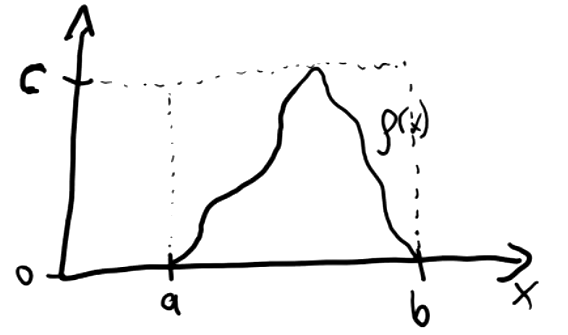
\includegraphics[width=0.4\textwidth]{av-methode}
\end{wrapfigure}
Die Annahme-Verwerfungs-Methode ist ein geometrischer Ansatz, der zufällig
Punkte in einem rechteckigen Bereich generiert, der die
\link{def:dichte}{Dichtefunktion} der gewünschten Verteilung einrahmt.
Notwendige Voraussetzung dafür ist, dass ein endlich großes, die Dichtefunktion
umgebendes Rechteck gefunden werden kann.

Die zufälligen Punkte werden durch skalierte, gleichverteilte Zufallszahlen
bestimmt. Liegt der Punkt unterhalb des Graphs der Dichtefunktion, wird der
X-Wert des Punkts ausgegeben. Damit entspricht die Wahrscheinlichkeit, dass ein
bestimmter Wert als Zufallszahl ausgegeben wird, genau dem Wert der
Wahrscheinlichkeitsdichte an diesem Punkt.

Der folgende Algorithmus gibt eine Folge von Zufallszahlen in der gewünschten
Verteilung aus:

\begin{algorithm}[h!]
\DontPrintSemicolon
\LinesNumbered

\While{1}{
  Erzeuge $x\sim U(a,b)$\;
  Erzeuge $y\sim U(0,1)$\;
  \If{$y\cdot c \le \rho(x)$}{
    gib $x$ aus\;
  }
}


\caption{Annahme-Verwerfungs-Methode}\label{algo:av-methode}
\end{algorithm}

\subsection{Importance-Sampling}

Die Annahme-Verwerfungs-Methode funktioniert dann besonders gut, wenn die Fläche
unter der Dichtefunktion im Vergleich zum einhüllenden Rechteck möglichst gering
ist. In diesem Fall liegen nur wenige Punkte oberhalb der Dichte und müssen
verworfen werden. Ist das einhüllende Rechteck im Vergleich jedoch sehr groß,
beispielsweise weil die Wahrscheinlichkeitsdichte sehr ungleich verteilt ist,
werden viele Punkte verworfen, sodass mehr Zeit für die Erzeugung einer festen
Anzahl an Zufallszahlen erforderlich ist.

Beim Importance-Sampling wird statt eines einhüllenden Rechtecks eine einhüllende
Funktion $h(x)$ verwendet, die weniger Platz als das Rechteck "`verschwendet"'.
Dafür ersetzen wir in Algorithmus \ref{algo:av-methode} die obere Schranke $c$
durch den Wert der Einhüllenden $h(x)$.

Da die Einhüllende $h(x)$ jedoch im Allgmeinen nicht konstant ist, müssen wir
diese Verzerrung korrigieren. Dafür generieren wir die x-Werte der zufälligen
Punkte in der Verteilung der Einhüllenden. Die Einhüllende $h(x)$ besitzt
folgende \link{def:dichte}{Dichte}:
\[H(z) = \frac{1}{\gamma}\cdot\int_a^z h(x) \mathrm{d}x\]
Die Konstante $\gamma = \int_a^b h(x)\mathrm{d}x$ stellt die Normiertheit sicher.

Durch die Inverse $H^{-1}$ der Verteilungsfunktion können mit der
\link{satz:inversionsm}{Inversionsmethode} der Einhüllenden entsprechend
verteilte Zufallszahlen erzeugt werden (da $h(x)$ frei gewählt werden kann, ist
das Invertieren in der Regel kein Problem).

Der entsprechende Algorithmus sieht dann so aus:

\begin{algorithm}[h!]
\DontPrintSemicolon
\LinesNumbered

\While{1}{
  Erzeuge $u\sim U(a,b)$\;
  Setze $x = H^{-1}(u)$\;
  Erzeuge $y\sim U(0,1)$\;
  \If{$y\cdot h(x) \le \rho(x)$}{
    gib $x$ aus\;
  }
}

\caption{Annahme-Verwerfungs-Methode mit Importance Sampling}\label{algo:av-methode-is}
\end{algorithm}

\section{Box-Müller-Polarmethode}

TODO


  \chapter{Markov-Ketten}
  Markov-Ketten dienen zur Beschreibung von Prozessen, deren zukünftiger Zustand
nur durch den letzten Zustand bestimmt wird. Markov-Prozesse werden darum auch
als "`gedächtnislos"' bezeichnet.

\begin{definition}{Stochastischer Prozess}{stochp}
Sei $T=\N_0$ und $S \subset\R$. Für jedes $t\in T$ sei $X_t$ eine
\link{def:zvar}{Zufallsvariable} mit Zustandsraum $S$. Dann heißt die Familie
\[
\big(X_t\big)_{t\in T}
\]
\defw{stochastischer Prozess} mit Zustandsraum $S$ und diskreter Zeit. Ist
$T = [0, \infty)$ handelt es sich um einen \defw{stetigen stochastischen Prozess}.
\end{definition}

\begin{definition}{Markov-Kette}{mk}
Ein stochastischer Prozess $\big(X_t\big)_{t\in \N_0}$ mit Zustandsraum $S$
heißt \defw{Markov-Kette} falls für alle $n\in\N_0$ und $k,l,x_0,x_1,...,x_n \in S$
gilt:
\[
P\big(X_{n+1} = l | X_{n}=k, X_{n-1}=x_{n-1},...,X_0=x_0\big) =
P\big(X_{n+1}=l|X_n=k\big)
\]
Diese Wahrscheinlichkeit heißt Übergangswahrscheinlichkeit und wird mit $p(k,l)$
bezeichnet.
\end{definition}

Die Definition der Markov-Kette beschreibt genau die Eigenschaft der
"`Gedächtnislosigkeit"': Die Wahrscheinlichkeit, in den nächsten Zustand zu
wechseln hängt lediglich davon ab, wo man sich gerade befindet (und nicht von
den Schritten davor).

\begin{definition}{Übergangsmatrix einer Markovkette}{mk-matr}
Sei $(X)_{n\in N_0}$ eine \link{def:mk}{Markovkette} mit Zustandsraum $S$. Die
Übergangswahrscheinlichkeiten $p(i,j)$ mit $i,j\in S$ lassen sich als Matrix
anordnen:
\[
\Pi = \big(p(i,j)\big)_{i,j\in S}
\]
Diese Matrix wird als \defw{Übergangsmatrix} der Markov-Kette bezeichnet.
\end{definition}

Jede Zeile der Übergangsmatrix enthält die Wahrscheinlichkeiten, in den Zustand
der jeweiligen Spalte überzugehen. Die Matrix ist eine sogenannte
\defw{stochastische Matrix}, das heißt alle Einträge besitzen Werte zwischen $0$
und $1$ und die Summe jeder Zeile ist $1$.

\begin{definition}{Verteilung einer Markovkette}{mk-vert}
Sei $(X)_{n\in N_0}$ eine \link{def:mk}{Markovkette} mit Zustandsraum $S$. Dann
heißt der Zeilenvektor mit $m\in \N_0$
\[
\pi_m = \big(P(X_m=s_1), ...,P(X_m=s_n)\big),\ s_1, ..., s_n \in S
\]
Verteilung der Markovkette zur Zeit $m$.
\end{definition}

Die Komponente einer Verteilung $\pi$ für einen Zustand $s$ wird mit $\pi(s)$
bezeichnet.

\begin{theorem}{Berechnung einer Markovkette}{mk-ber}
Sei $S$ eine diskrete Menge, $\Pi = \big(p(k,l)\big)_{k,l\in S}$ eine
stochastische Matrix auf $S$ und $\pi_0 = \big(p_0(k)\big)$ die
\link{def:mk-vert}{Verteilung} der Zustände zu Beginn der Betrachtung. Dann ist
die Verteilung $\pi_n$ nach $n$ Schritten berechenbar durch
\[
\pi_n = \pi_0\cdot\Pi^n
\]
Die Matrix $\Pi^n$ gibt die Wahrscheinlichkeit an, in $n$ Schritten von
Zustand $i$ in Zustand $j$ überzugehen.
\end{theorem}

Damit hängt die Wahrscheinlichkeit, sich nach einer festen Anzahl an Schritten
in einem bestimmten Zustand zu befinden, neben den Übergangswahrscheinlichkeiten
$\Pi$ nur von der Anfangsverteilung ab.

\begin{theorem}{Chapman-Kolmogorow-Gleichung}{chapman}
Sei $(X)_{n\in N_0}$ eine Markovkette mit Zustandsraum $S$. Dann kann die
Wahrscheinlichkeit, in $n+m$ Schritten von Zustand $i$ in Zustand $k$ zu
wechseln gleich der Summe der Pfade über alle möglichen Zwischenstationen:
\[
P(X_{n+m}=k|X_0=i) = \sum_{j\in S}P(X_{n+m}=k|X_n=j)\cdot P(X_n=j|X_0=i)
\]
\end{theorem}

Das lässt sich durch die Definition der Matrixmultiplikation zeigen
(\href{https://de.wikipedia.org/wiki/Chapman-Kolmogorow-Gleichung}{Wikipedia}).

\section{Eigenschaften}

\begin{definition}{Pfad}{mk-pfad}
Ein konkreter Folge von Zuständen einer Markovkette $(X)_{n\in N_0}$ wird
als \defw{Pfad} bezeichnet.
\end{definition}

\subsection{Zustandsklassen}

Die Zustände von Markovketten können zum Beispiel nach ihrer Erreichbarkeit
untereinander unterschieden werden.

\begin{definition}{Interaktionsgraph}{mk-igraph}
Sei $(X)_{n\in N_0}$ eine Markovkette mit Zustandsraum $S$. Der gerichtete Graph
$G=(V,E)$ mit Kanten $V=S$ und $E = \{(x,y) \in S\times S\ |\ p(x,y) \ne 0\}$ wird
als \defw{Interaktionsgraph} bezeichnet.
\end{definition}

Der Interaktionsgraph beschreibt also die direkten
Verbindungen der Zustände im Zustandsraum.

\begin{definition}{Erreichbarkeit}{mk-erreichbar}
Sei $(X)_{n\in N_0}$ eine Markovkette mit Zustandsraum $S$. Ein Zustand $y\in S$
heißt erreichbar von $x\in S$, falls es ein $n>0$ gibt, sodass gilt:
\[
P(X_n=y|X_0=x) > 0
\]
Erreichbarkeit kann auch durch die \link{def:mk-matr}{Übergangsmatrix} $\Pi$
definiert werden:
\[
\exists n\in\N: \Pi^n(x,y) \ne 0
\]
\end{definition}

Ist $y$ von $x$ erreichbar, existiert im Interaktionsgraph ein Pfad von $x$ zu
$y$. Dieser Pfad muss nicht direkt sein, sondern kann auch über andere Zustände
führen. Wir verwenden für diese Erreichbarkeit die Schreibweise $x\to y$.

\begin{definition}{Verbundene Zustände}{mk-verb}
Sei $S$ der Zustandsraum einer Markovkette. Die Zustände $x,y\in S$ heißen
\defw{verbunden}, wenn gilt:
\[
x\to y \land y \to x
\]
Verbundene Zustände werden durch das Zeichen $\lr$ gekennzeichnet
($x \lr y$).
\end{definition}

Die Verbundenheit von Zuständen ist eine Relation, die \emph{reflexiv} (jeder
Zustand ist mit sich selbst verbunden), \emph{symmetrisch} (verbundene
Zustände sind auch in der "`Gegenrichtung"' verbunden) und \emph{transitiv}
(sind $a$ mit $b$ und $b$ mit $c$ verbunden, ist auch $a$ mit $c$
verbunden). Damit ist die Relation $\lr$ eine Äquivalenzrelation\more{mfnf-ä-rel}.
Das bedeutet insbesondere, dass die Zustandsmenge $S$ durch die Verbundenheitsrelation in
Äquivalenzklassen zerlegt wird, in denen jeder Zustand mit jedem anderen Zustand
verbunden ist.

Zwischen Äquivalenzklassen kann sich nicht beliebig bewegt werden; insbesondere
kann eine einmal verlassene Klasse nicht wieder erreicht werden. (Gäbe es einen
"`Weg zurück"', wären auch jedes Paar von Zuständen aus beiden Klassen
miteinander verbunden. Das ist ein ein Widerspruch, denn dann müssten diese
Zustände ja in \emph{einer} gemeinsamen Äquivalenzklasse liegen.)

Um die Zustände einer Markovkette zu klassifizieren, beginnt man bei einem
beliebigen Zustand und bestimmt dessen transitive Hülle bezüglich $\lr$, also
alle Zustände die mit dem gewählten Zustand verbunden (nicht nur erreichbar!)
sind. Damit ist eine Klasse der Markovkette gefunden. Dieses Vorgehen
wird dann mit nicht klassifizierten Zuständen wiederholt, bis alle Zustände
klassifiziert sind.

\begin{example}{Bestimmung der Zustandsklassen}{}
Gesucht sind die Zustandsklassen eine Markovkette mit folgendem Interaktionsgraph:

\begin{centering}
\begin{tikzpicture}
  \node[v] (1) at (2,1) {1};
  \node[v] (2) at (4,2) {2};
  \node[v] (3) at (6,2) {3};
  \node[v] (6) at (5,0) {6};
  \node[v] (4) at (8,1) {4};
  \node[v] (5) at (10,1) {5};

  \draw[e] (1) to[loop above] ();
  \draw[e] (6) -- (1);
  \draw[e] (6) -- (3);
  \draw[e] (2) to[bend right] (3);
  \draw[e] (3) to[bend right] (2);
  \draw[e] (2) to[loop above] ();
  \draw[e] (2) -- (6);
  \draw[e] (6) -- (4);
  \draw[e] (4) to[bend left] (5);
  \draw[e] (5) to[bend left] (4);
\end{tikzpicture}
\end{centering}

Zustand 1 ist mit keinen weiteren Zuständen verbunden.
Zustand 2 ist mit Zuständen 3 und 6 verbunden, aber z.B. nicht mit Zustand 4
oder 1, da von dort aus kein Weg zurück führt.
Zustand 4 ist mit Zustand 6 verbunden.
Damit sind alle Zustände eingeordnet und die Zerlegung der Zustände ist:
\[
S_{/\lr} = \{\{1\}, \{2,3,6\}, \{4, 5\}\}
\]
\end{example}

Die \link{def:mk-erreichbar}{Erreichbarkeit von Zuständen} können wir auf die
Äquivalenzklassen übertragen:
\begin{definition}{Ordnung von Zustandsklassen}{mk-ord}
Sei $S$ der Zustandsraum einer Markovkette, der durch die Verbundenheitsrelation
$\lr$ in Klassen $S_{/\lr}=\{G_1, G_2,...,G_n\}$ zerlegt wird. Auf diesen
Klassen definieren wir folgende Relation:
\[
\preceq\ =\{(G_i, G_j)\ |\ \exists s_i\in G_i, s_j\in G_j: s_i\to s_j\}\ \subseteq\ S_{/\lr}\times S_{/\lr}
\]
Die Relation bildet eine partielle Ordnung\more{mfnf-o-rel}, ist also reflexiv, anti-symmetrisch und transitiv. Für
$G_i\preceq G_j$ schreiben wir auch $G_i\to G_j$.
\end{definition}

Die so definierte Ordnung ist jedoch im Allgemeinen nicht \emph{total}, da nicht
für jedes Paar von Zustandsklassen definiert sein muss, ob $G_i\preceq G_j$ oder
$G_j \preceq G_i$ gilt. Das ist zum Beispiel der Fall, wenn die Klassen nicht
miteinander verbunden sind, also im Interaktionsgraphen unverbundene Subgraphen
bilden oder wenn zwei unverbundene Klassen in einem dritten Zustand
"`zusammenlaufen"'.

\begin{definition}{Abgeschlossene Klasse}{mk-abg}
Sei $G$ eine Zustandsklasse einer Markovkette. $G$ heißt \defw{abgeschlossen},
wenn es keine Klasse gibt, die von $G$ erreicht werden kann:
\[
\nexists H\ne G: G\preceq H
\]
\end{definition}

Abgeschlossene Klassen werden zusätzlich nach der Anzahl ihrer Zustände
unterschieden:

\begin{definition}{Absorbierende Klasse/Markovkette}{mk-abs}
Sei $(X)_{n\in N_0}$ eine Markovkette. Ist $G$ eine \link{def:mk-abg}{abgeschlossene Klasse}
mit $|G|=1$, so heißt die Klasse $G$ \defw{absorbierend}.

Sind alle abgeschlossenen Klassen absorbierend, so heißt die
Markovkette \defw{absorbierend}.
\end{definition}

Sind alle Zustände einer Markovkette miteinander verbunden, gibt es nur eine
Äquivalenzklasse:
\begin{definition}{Irreduzibilität}{mk-irred}
Sei $(X)_{n\in N_0}$ eine Markovkette mit Zustandsraum $S$, der durch die
Verbundenheitsrelation $\lr$ in die Menge $S_{/\lr}$ zerlegt wird. Existiert nur
eine einzige Klasse, das heißt es gilt
\[
S_{/\lr}\ = \{S\}
\]
heißt die Markovkette \defw{irreduzibel}.
\end{definition}

Das ist genau der Fall, dass alle Zustände mit allen anderen Zuständen verbunden
sind, sodass genau eine Klasse besteht.

\begin{lemma}
Die Klasse $S$ einer irreduziblen Markovkette ist abgeschlossen.
\end{lemma}
 
\subsection{Rückkehreigenschaften}

In diesem Abschnitt werden Zustände von Markovketten bezüglich ihres
Rückkehrverhaltens untersucht\more{wiki-mk-properties}.

\begin{definition}{Rückkehrzeit}{mk-rueckk}
Sei $(X)_{n\in N_0}$ eine Markovkette mit Zustandsraum $S$ und $y\in S$
\link{def:mk-rekurr}{rekurrent} und der Startzustand $X_0$ der Markovkette.
Dann heißt
\[
T_y = min\{n>0:\ X_n = y\}
\]
die (zufällige) \defw{Rückkehrzeit} in den Zustand $y$. Zusätzlich bezeichnet
\[
M_y = \{k>0: P(T_y=k|X_0=y > 0\}
\]
die Menge der Zeitschritte, in denen ausgehend von $y$ wieder $y$ erreicht
werden kann.
\end{definition}

\begin{definition}{Periode eines Zustands}{mk-periode}
Sei $(X)_{n\in N_0}$ eine Markovkette mit Zustandsraum $S$ und $y\in S$ ein
Zustand, der \emph{nur} in $M_y=\{d, 2d, 3d, ...\}$ Schritten erreicht werden
kann, so heißt
\[
d = \mathrm{ggT}(M_y)
\]
die \defw{Periode} des Zustands $y$.
\end{definition}

\begin{definition}{Aperiodischer Zustand, aperiodische Markovkette}{mk-aperiod}
Sei $y$ ein Zustand einer Markovkette. Besitzt dieser Zustand die Periode 1, so
heißt $y$ \defw{aperiodisch}.

Sind alle Zustände einer Markovkette aperiodisch, heißt die Markovkette
\defw{aperiodisch}.
\end{definition}

\begin{definition}{Ergodische Markovkette}{mk-ergod}
Ist eine Markovkette mit endlich vielen Zuständen \link{def:mk-irred}{irreduzibel} und
\link{def:mk-aperiod}{aperiodisch}, so heißt sie \defw{ergodisch}.
\end{definition}

Die Zustände eines \link{def:stochp}{stochastischen Prozess} können danach
unterschieden werden, ob man in jedem Fall zu dem Zustand, in dem man gestartet
ist, zurückkehren kann (rekurrent) oder nicht (transient)
\more{brilliant-transience-recurrence}:

\begin{definition}{Rekurrenter Zustand}{mk-rekurr}
Sei $y$ ein Zustand einer Markovkette. Dann heißt $y$ \defw{rekurrent}, wenn
es für jeden von $y$ aus \link{def:mk-erreichbar}{erreichbaren} Zustand einen
Weg zurück zu $i$ gibt.
\end{definition}

\begin{definition}{Transienter Zustand}{mk-trans}
Sei $y$ ein Zustand einer Markovkette. Dann heißt $y$ \defw{transient}, wenn $y$
nicht rekurrent ist.
\end{definition}

Per Definition besteht bei transienten Zuständen die "`Gefahr"', nicht mehr in
diese zurückkehren zu können. Auf lange Sicht sind transiente Zustände daher nur
Zwischenzustände.

Die Eigenschaften \link{def:mk-rekurr}{Rekurrenz} und
\link{def:mk-trans}{Transienz} sind Klasseneigenschaften: Besitzt ein Zustand
eine dieser Eigenschaften, so auch alle anderen Zustände der Klasse. (Innerhalb
einer Klasse sind schließlich immer alle Zustände miteinander verbunden, es gibt
also immer einen Weg zurück zum Startzustand. Damit "`überträgt"' sich die
Transienz bzw. Rekurrenz eines Zustands auf die gesamte Klasse.)

\begin{lemma}
Jede \link{def:mk-abg}{abgeschlossene} Klasse ist rekurrent.

Begründung: Eine abgeschlossene Klasse kann nur betreten, aber nicht mehr
verlassen werden. Somit sind nur Zustände der Klasse erreichbar, sodass immer
zum Startzustand zurückgekehrt werden kann.
\end{lemma}

\begin{example}{Transiente/Rekurrente Zustandsklassen}{mk-tr-rek}
Gegeben sei eine Markovkette mit folgendem Interaktionsgraph:

\begin{tikzpicture}
  \node[v] (1) at (2,1) {1};
  \node[v] (2) at (4,2) {2};
  \node[v] (3) at (6,2) {3};
  \node[v] (6) at (5,0) {6};
  \node[v] (4) at (8,1) {4};
  \node[v] (5) at (10,1) {5};

  \draw[e] (1) to[loop above] ();
  \draw[e] (6) -- (1);
  \draw[e] (6) -- (3);
  \draw[e] (2) to[bend right] (3);
  \draw[e] (3) to[bend right] (2);
  \draw[e] (2) to[loop above] ();
  \draw[e] (2) -- (6);
  \draw[e] (6) -- (4);
  \draw[e] (4) to[bend left] (5);
  \draw[e] (5) to[bend left] (4);
\end{tikzpicture}

Die Markovkette besitzt die Zustandsklassen $S_{1}=\{1\}$, $S_{2,3,6} =\{2,3,6\}$
und $S_{4,5}=\{4, 5\}$. Zustand 1 ist rekurrent, da alle erreichbaren Zustände
(also nur der Zustand selbst) wieder einen Pfad zurück zum Zustand 1 besitzen.
Wenn man in 1 startet, kann es also nicht passieren, dass man nicht mehr dahin
zurückkommt.
Die Klasse $S_{2,3,6}$ ist transient, da man von dort aus auch in die Klassen
$S_1$ und $S_{4,5}$ kommen kann, von denen jedoch kein Pfad zurück in die
"`Startklasse"' führt. Die Klasse $S_{4,5}$ ist rekurrent, da sie (wie auch
$S_1$) nicht verlassen werden kann.
\end{example}

  \section{Langzeitverhalten}

\newcommand{\stat}{\underline{\pi}} % stationäre Wahrscheinlichkeit

Dieser Abschnitt beschäftigt sich mit der \link{def:mk-vert}{Verteilung der
Markovkette} nach unendlich vielen Schritten.

\textbf{Achtung: Die hier verwendete
Notation weicht zum Teil deutlich von den Vorlesungsvideos ab.}

\begin{definition}{Stationäre Verteilung}{mk-stat}
Sei $(X)_{n\in N_0}$ eine Markovkette mit \link{def:mk-matr}{Übergangsmatrix}
$\Pi$ und endlichem Zustandsraum $S$. Dann heißt die
\link{def:mk-vert}{Verteilung} $\stat$ \defw{stationäre Verteilung},
wenn gilt:
\[
\stat\cdot\Pi = \stat
\]
\end{definition}

Gelangt oder startet man in einer stationären Verteilung, ändert sich die
Wahrscheinlichkeit, sich in einem Zustand zu befinden, nicht mehr.

\subsection{Ergodische Markovketten}

\begin{theorem}{Hauptsatz für ergodische Markovketten}{ergod}
Sei $(X)_{n\in N_0}$ eine \link{def:mk-ergod}{ergodische} Markovkette mit
\link{def:mk-matr}{Übergangsmatrix} $\Pi$ und $y$ ein Zustand der Markovkette
mit \link{def:mk-rueckk}{Rückkehrzeit} $T_y$. Dann
besitzt die Markovkette \emph{genau} eine stationäre Verteilung $\stat$
für die gilt:
\[
\lim_{n\to\infty}\Pi(X_n = y) = lim_{n\to\infty}\Pi^n(x, y) = \stat(y)
\]
Weiterhin existiert ein Zusammenhang zwischen der erwarteten Rückkehrzeit und
der stationären Verteilung:
\[
\stat(y) = \frac{1}{\E(T_y|X_0=y)}
\]
\end{theorem}

Je weiter eine ergodische Markovkette läuft, desto mehr nähert sich die
Wahrscheinlichkeitsverteilung an die stationäre Verteilung an. Die stationäre
Verteilung gibt – zumindest auf lange Sicht – an, mit welcher Wahrscheinlichkeit
man sich in den jeweiligen Zuständen befindet.

Die stationäre Verteilung einer ergodischen Markovkette kann berechnet
werden. Dafür nutzt man die Tatsache, dass die stationäre Verteilung (per
Definition) ein Eigenvektor\more{mfnf-ew-ev} der Übergangsmatrix. Zusätzlich
muss wird eine Gleichung eingefügt, die die Normierung der stationären
Verteilung auf 1 sicherstellt. Es ergibt sich folgendes
lineares Gleichungssystem:
\begin{equation}\label{eq:stat-lgs}
\begin{pmatrix}
\Pi_{00}-1 & \Pi_{10} & \ldots & \Pi_{j0} \\
\Pi_{01} & \Pi_{11}-1 &        & \Pi_{j1} \\
\vdots   &            & \ddots & \vdots \\
\Pi_{0i} & \Pi_{1i} & \ldots &   \Pi_{ji}-1 \\
    1    &     1    & \ldots &   1
\end{pmatrix}\cdot \vec{\stat} = \begin{pmatrix}0\\0\\\vdots\\0\\1\end{pmatrix}
\end{equation}
Wichtig ist auch, dass die Matrix $\Pi$ transponiert aufgeschrieben, da eine
Spalte der Matrix einer Gleichung entspricht.

\subsection{Nichtergodische Markovketten}

\newcommand{\lzv}{\Pi^\infty} % Langzeitverhalten

Bei Nichtergodischen Markovketten ist das Langzeitverhalten nicht so einfach
bestimmbar, da die stationäre Verteilung vom Startzustand abhängt. Das
Langzeitverhalten der Markovkette wird durch die Matrix $\lzv$ beschrieben,
die für jeden möglichen Startzustand die entsprechende Langzeitverteilung
angibt.

\medskip
Sei $(X)_{n\in N_0}$ eine Markovkette mit endlichem Zustandsram $S$ und
\link{def:mk-matr}{Übergangsmatrix} $\Pi$, wobei $T\subseteq S$ die Menge aller
\link{def:mk-trans}{transienten} Zustände ist. Es gelten die nachfolgende Regeln
zur Bestimmung des Langzeitverhaltens.

In einer \link{def:mk-abg}{abgeschlossenen} Klasse $C$ kann das
Langzeitverhalten als \link{def:mk-stat}{stationäre Verteilung}
$\stat^{(C)}$ der auf die Zustände in $C$ beschränkten Markovkette bestimmt
werden (vergleiche \eqref{eq:stat-lgs}):
\begin{equation}\label{eq:lzv-abg-abg}
  \forall x,y\in C: \lzv(x,y) = \stat^{(C)}(y)
\end{equation}
Da eine \link{def:mk-abg}{abgeschlossene} Klasse $C$ nicht
verlassen werden kann, gilt für $x\in C$ und $y \notin C$:
\begin{equation}\label{eq:lzv-abg-x}
  \lzv(x,y) = 0
\end{equation}
Damit ist das Langzeitverhalten der Startzustände in abgeschlossenen Klassen
bestimmt.

\medskip
Das Langzeitverhalten bei Start in einem \link{def:mk-trans}{transienten}
Zustand $t\in T$ muss die
Wahrscheinlichkeit der Absorption durch eine abgeschlossene Klasse $C$
berücksichtigt werden, die mit $p_{abs}(t,C)$ bezeichnet wird. Die
Absorptionswahrscheinlichkeit berechnet sich rekursiv als Wahrscheinlichkeit des
direkten Übergangs in die absorbierende Klasse plus die Wahrscheinlichkeit des
indirekten Übergangs mit einem zusätzlichen Schritt innerhalb der transienten
Klasse:
\[
p_{abs,t}(C) = \sum_{y\in C} \Pi(x,y) + \sum_{z\in T}\Pi(x,z)\cdot p_{abs,z} \\
\]
Für alle $t$ einer transienten Klasse entsteht so ein Gleichungssystem.

Die Wahrscheinlichkteit, bei Start in $t$ in $y\in S$ zu
enden, berechnet sich durch die Absorptionswahrscheinlichkeit verknüpft mit
der stationären Wahrscheinlichkeit $\stat^{(C)}$ innerhalb von $C$:
\begin{equation}\label{eq:lzv-trans-abg}
\lzv(x,y) = p_{abs,t}(C)\cdot\stat^{(C)}(y)
\end{equation}
Die Wahrscheinlichkeit, sich in einem \link{def:mk-trans}{transienten}
Zustand zu befinden, sinkt auf lange Sicht auf 0:
\begin{equation}\label{eq:lzv-trans-trans}
\forall x\in S, y\in T: \lzv(x, y) = 0
\end{equation}
Damit ist das Langzeitverhalten für den Start in einem transitiven Zustand
definiert.
Da in endlichen Markovketten alle abgeschlossenen Klassen rekurrent sind
\warn{Begründung bzw. Beweis fehlt}, sind
durch die obigen Definitionen das Langzeitverhalten bestimmt.

\begin{example}{Langzeitverhalten einer nichtergodischen Markovkette}{mk-lzv-nerg}
Gegeben sei folgende Markovkette:

\begin{minipage}{0.45\textwidth}
  \begin{tikzpicture}
    \node[v] (1) at (0,1.5) {1};
    \node[v] (2) at (-1.5,0) {2};
    \node[v] (3) at (0,0) {3};
    \node[v] (4) at (1.5,0) {4};

    \draw[e] (1) to[loop above] ();
    \draw[e] (2) to[loop below] ();
    \draw[e] (3) to[loop below] ();
    \draw[e] (4) to[loop below] ();
    \draw[e] (1) -- (2);
    \draw[e] (1) -- (3);
    \draw[e] (1) -- (4);
    \draw[e] (2) to[bend left] (3);
    \draw[e] (3) to[bend left] (2);
  \end{tikzpicture}
\end{minipage}
\begin{minipage}{0.45\textwidth}
  \[\Pi = \begin{pmatrix}
    0.1 & 0.4 & 0.3 & 0.2 \\
     0  & 0.2 & 0.8 &  0  \\
     0  & 0.9 & 0.1 &  0  \\
     0  &  0  &  0  &  1
  \end{pmatrix}\]
\end{minipage}

Die Markovkette ist nicht \link{def:mk-irred}{irreduzibel}, da mehr als eine
Klasse existiert ($S_{/\lr} = {S_1, S_{2,3}, S_{4}}$), Satz \ref{satz:ergod}
kann also nicht angewandt werden.

\medskip
Da Klasse $S_4$ abgeschlossen und Zustand 4 absorbierend ist, ergibt sich als
Sonderfall von \eqref{eq:lzv-abg-abg} und \eqref{eq:lzv-abg-x} folgende
Verteilung:
\[\begin{pmatrix}0 & 0 & 0 & 1\end{pmatrix}\]

Klasse $S_{2,3}$ ist abgeschlossen. Die stationäre Verteilung $\stat^{(S_{2,3})}$
ergibt sich als Lösung des Gleichungssystems (Vergleiche \eqref{eq:stat-lgs})
und bestimmt $\lzv(2..3, 2..3)$:
\[
\begin{pmatrix}
0.2 -1 & 0.9     \\
0.8    & 0.1 - 1 \\
   1   &  1
\end{pmatrix}\cdot \vec{\stat}^{(S_{2,3})} = \begin{pmatrix}0\\0\\1\end{pmatrix}
\iff \vec{\stat}^{(S_{2,3})} =
\renewcommand\arraystretch{1.3}
\begin{pmatrix}0.53\\0.47\end{pmatrix}
\]

Zustand 1 ist transient, damit gilt $\lzv(1,1) = 0$
(\eqref{eq:lzv-trans-trans}). Als Zwischenergebnis bestimmen wir die
Absorptionswahrscheinlichkeiten $p_{abs,1}(S_{2,3})$ und $p_{abs,1}(S_{4})$:
\begin{align*}
p_{abs,1}(S_{2,3}) &=&  0.4 + 0.3 + 0.1 \cdot p_{abs,1}(S_{2,3}) & \implies
p_{abs,1}(S_{2,3}) = \frac{0.7}{0.9} = 0.78  \\
p_{abs,1}(S_{4})   &=&  0.2 + 0.1 \cdot p_{abs,1}(S_4) &\implies
p_{abs,1}(S_4) =\frac{0.2}{0.9} = 0.22
\end{align*}
Durch Anwendung von Gleichung \eqref{eq:lzv-trans-abg} ergibt sich:
\begin{align*}
\lzv(1,2) &=& p_{abs,1}(S_{2,3}) &\cdot\stat^{(S_{2,3})}(2) &= 0.41 \\
\lzv(1,3) &=& p_{abs,1}(S_{2,3}) &\cdot\stat^{(S_{2,3})}(3) &= 0.37 \\
\lzv(1,4) &=& p_{abs,1}(S_4)     &\cdot\stat^{(S_4)}    (4) &= 0.22
\end{align*}
Damit sind alle Einträge der Matrix $\lzv$ bestimmt:
\[
\lzv = \begin{pmatrix}
   0  & 0.41 & 0.37 & 0.22 \\
   0  & 0.53 & 0.47 &  0   \\
   0  & 0.53 & 0.47 &  0   \\
   0  &  0   &  0   &  1
\end{pmatrix}
\]
Als Probe kann sichergestellt werden, dass die Matrix stochastisch ist, sich
also die Einträge jeder Zeile zu 1 summieren.
\end{example}


  \printbibliography
\end{document}
